\chapter{Results} \label{chapResults}
\section{3D reconstructions}
Here we perform 3D reconstructions on a variety of locations. We find that the qualitative results look really good. 

\begin{figure}
    \centering
    \includegraphics[width=\textwidth]{example-image-a}
    \caption{Caption}
    \label{fig:3d_reconstrction}
\end{figure}

\begin{figure}
    \centering
    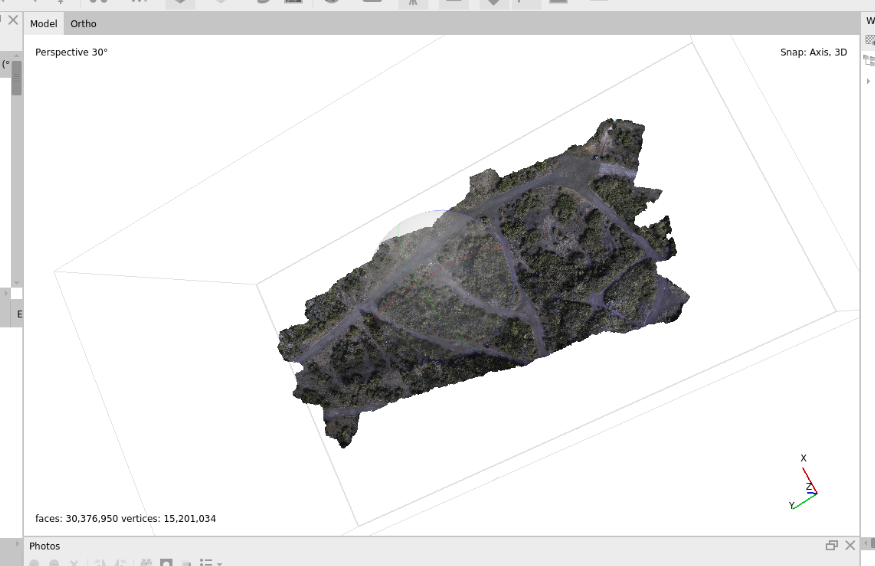
\includegraphics[width=\textwidth]{figs/results/3d_reconstruction.png}
    \caption{An example 3D reconstruction developed using Agisoft, a commercial structure from motion software.}
    \label{fig:3d_reconstrction}
\end{figure}

\section{Image-based predictions}
\subsection{Semantic segmentation}
\begin{figure*}[h!]
   \centering
   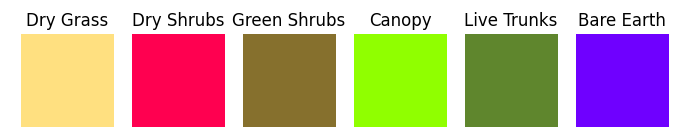
\includegraphics[width=0.5\textwidth]{figs/results/semantic_segmentation/Gascola/safeforest_all_classes_flat.png}
   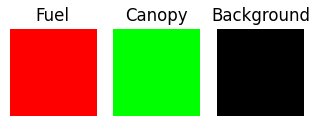
\includegraphics[width=0.25\textwidth]{figs/results/semantic_segmentation/Gascola/safeforest_classmap_compressed_flat.png}
   \includegraphics[width=0.80\textwidth]{figs/results/semantic_segmentation/Gascola/000000_rgb_img.png}
   \vspace{0pt}
   \includegraphics[width=0.80\textwidth]{figs/results/semantic_segmentation/Gascola/000005_rgb_img.png}
   \vspace{0pt}
   \includegraphics[width=0.80\textwidth]{figs/results/semantic_segmentation/Gascola/000010_rgb_img.png}
   \vspace{0pt}
   \includegraphics[width=0.80\textwidth]{figs/results/semantic_segmentation/Gascola/000015_rgb_img.png}
   \vspace{0pt}
   \caption{
   Qualitative semantic mapping results from the test set. The results are shown both for the predicted classes and the aggregated ones, with colors visualized in the top rows.
   White regions in the ground truth represent areas that were ambiguous to the human annotator. Overall the predictions match the ground truth well and boundaries are well-defined. Note that many regions of confusions, such as canopy-to-trunk and green shrub to canopy, fall within the same coarse classes for our mapping purposes.
   }
   \label{fig:results_semantic_seg_qualitative}                %% Etiqueta para la figura entera
\end{figure*}
\subsection{Tree detection}

\begin{figure}
    \centering
    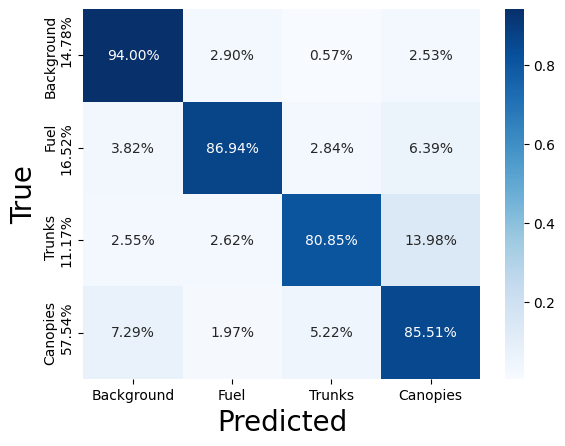
\includegraphics[width=\textwidth]{figs/results/confusion_matrix.png}
    \caption{Confusion matrix semantics}
    \label{fig:res_confusion_matrix}
\end{figure}

\section{Geospatial map predictions}
\subsection{Semantic segmentation}
For gascola and maybe 
\subsection{Tree detection}

\begin{figure}[h]
    \subfloat{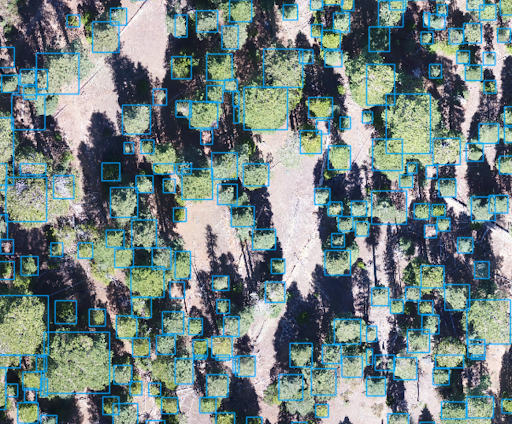
\includegraphics[width=0.45\textwidth]{figs/results/tree_detections/emerald_point_tree_detections.png}}
    \hfill
    \subfloat{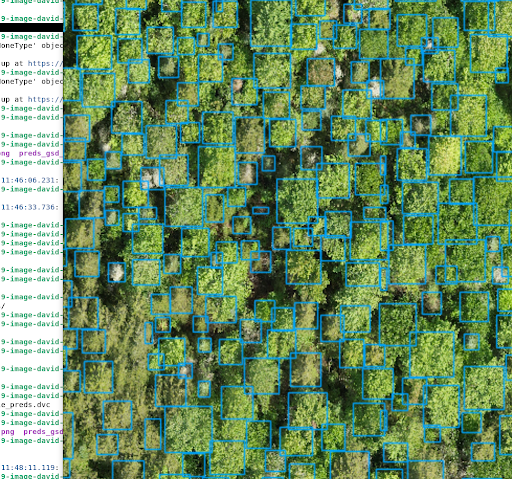
\includegraphics[width=0.45\textwidth]{figs/results/tree_detections/stowe_anew_detections.png}}
    \caption{Visualizations of the proposed planning method on two different data images.}
    \label{fig:res_unpairqual}
\end{figure}



%\begin{figure}
%    \centering
%    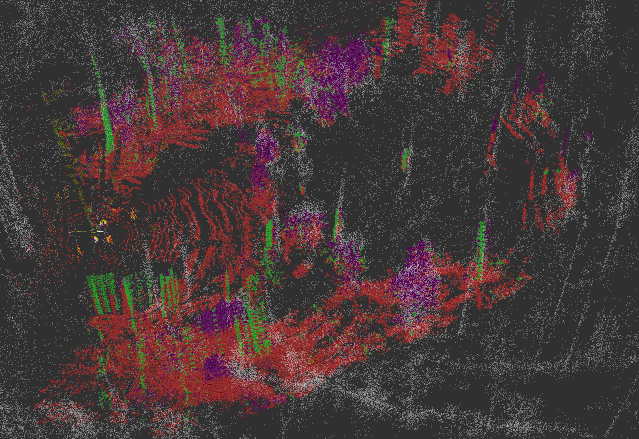
\includegraphics[width=\textwidth]{figs/results/semantic_cloud3_cropped.png}
%    \caption{Semantics cloud}
%    \label{fig:res_semantic_cload}
%\end{figure}


\section{Unsupervised feature extraction and predictions}

\begin{figure}
    \centering
    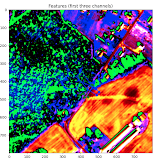
\includegraphics[width=\textwidth]{figs/results/feature_extraction/Screenshot from 2023-05-19 10-03-18.png}
    \caption{Unsupervised features extracted from the data}
    \label{fig:res_unsupervised_feature_qual}
\end{figure}

\begin{figure}
    \centering
    \includegraphics[width=\textwidth]{example-image-a}
    \caption{Random satellite predictions using the features}
    \label{fig:sat_predictions}
\end{figure}


\section{Informative path planning}

\begin{figure}[h]
    \subfloat{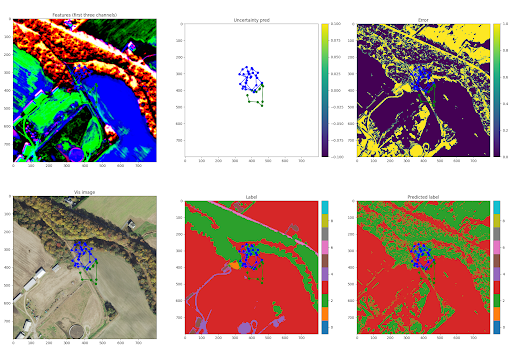
\includegraphics[width=0.45\textwidth]{figs/results/ipp/unpaired_qual_1 (1).png}}
    \hfill
    \subfloat{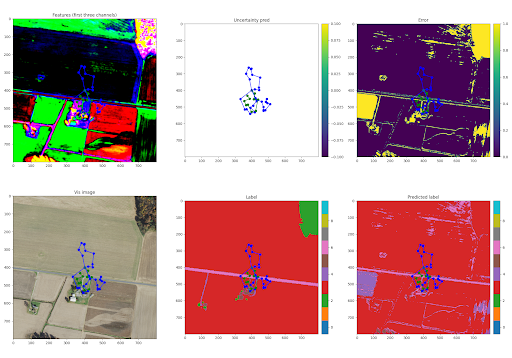
\includegraphics[width=0.45\textwidth]{figs/results/ipp/unpaired_qual_2 (1).png}}
    \caption{Visualizations of the proposed planning method on two different data images.}
    \label{fig:res_unpairqual}
\end{figure}


\begin{figure}[h]
    \subfloat{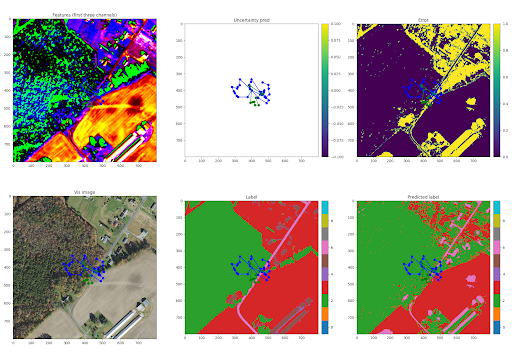
\includegraphics[width=0.45\textwidth]{figs/results/ipp/paired_qual_GBS-IPP (1).png}}
    \hfill
    \subfloat{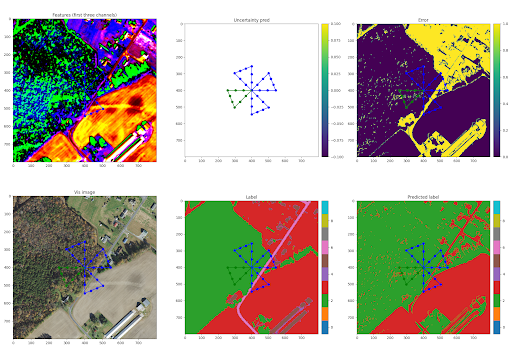
\includegraphics[width=0.45\textwidth]{figs/results/ipp/paired_qual_pizza (1).png}}
    \caption{A comparison of the proposed method with a baseline}
    \label{fig:res_pairedqual}
\end{figure}

\begin{figure}[h]
    \subfloat{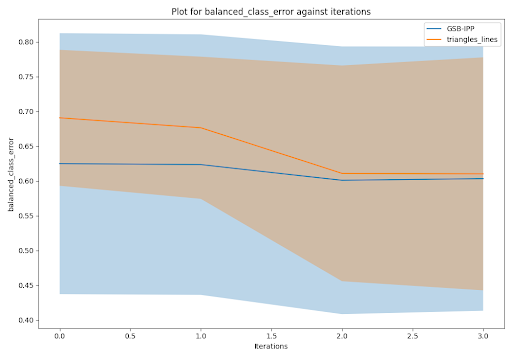
\includegraphics[width=0.3\textwidth]{figs/results/ipp/error (2).png}}
    \hfill
    \subfloat{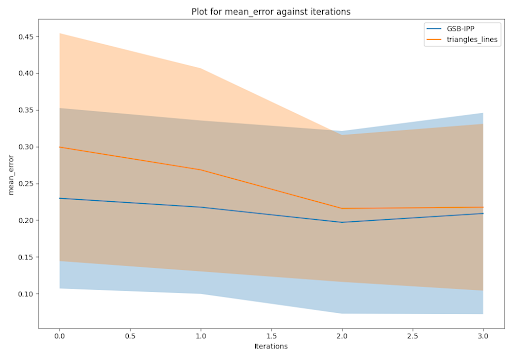
\includegraphics[width=0.3\textwidth]{figs/results/ipp/balanced_error (2).png}}
    \hfill
    \subfloat{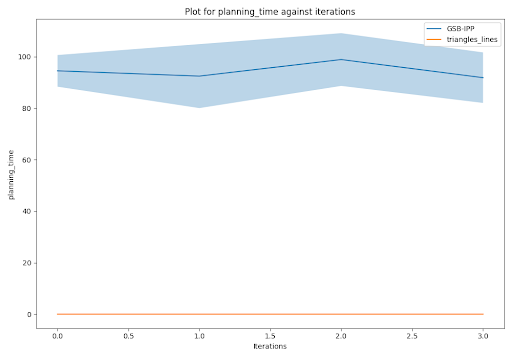
\includegraphics[width=0.3\textwidth]{figs/results/ipp/timing_result (1).png}}
    \caption{Quantitative statistics for IPP}
    \label{fig:res_ipp_quant}
\end{figure}